\comment{
\begin{figure}
(a) DDMS: show state machine, with databases as states and updates as transitions.

(b) DBMS: database sits and waits for queries to arrive; answers them.

(c) Data stream processor: Set of sitting queries; a stream of data passes by.

\caption{Data management systems architectures: DDMS vs. DBMS vs. data stream processors.}
\end{figure}
}

\begin{figure}
\begin{center}
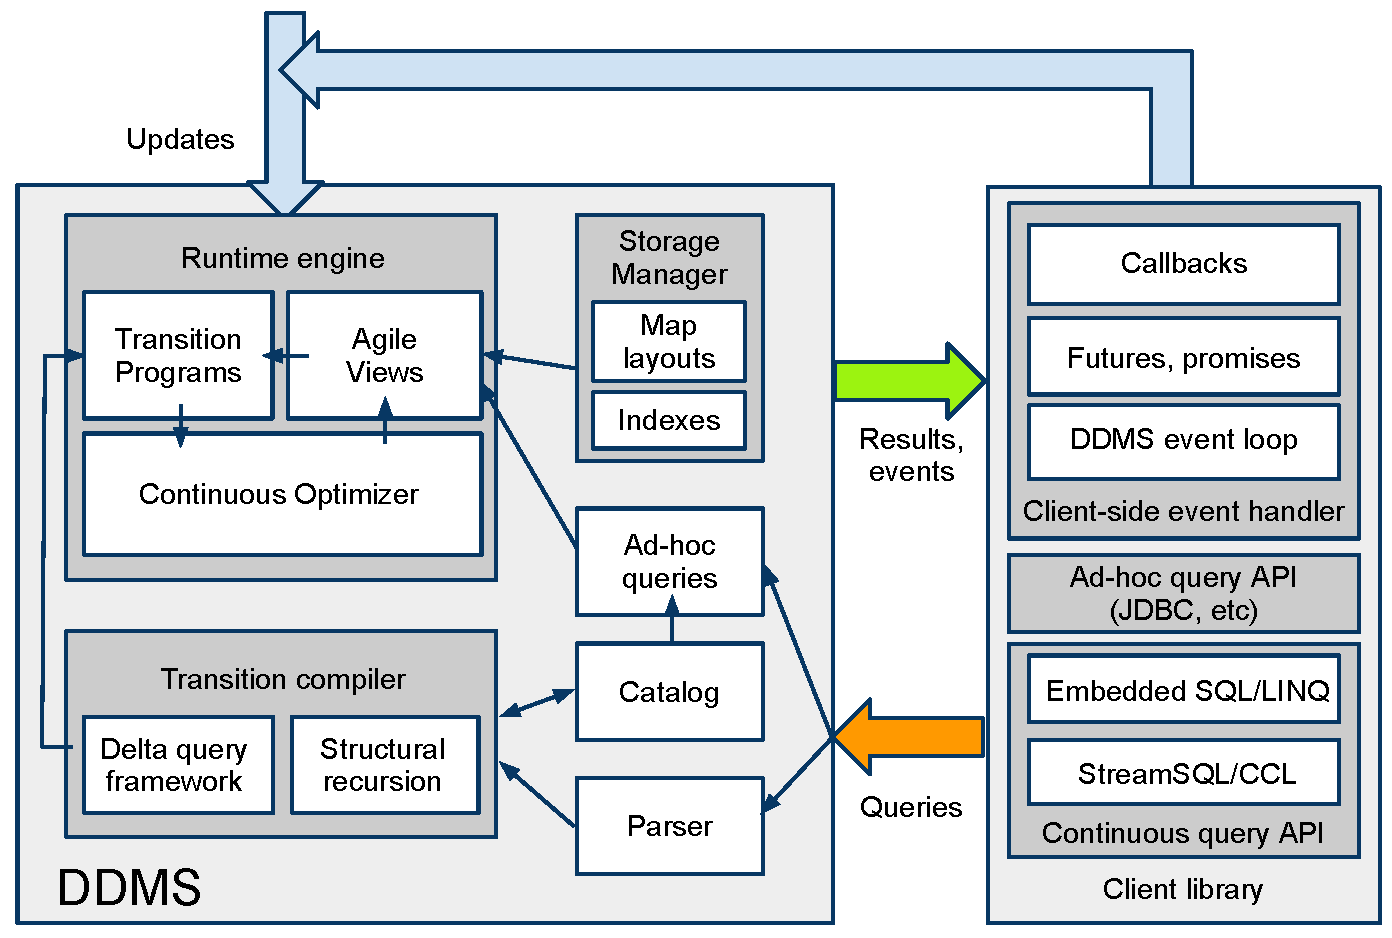
\includegraphics[width=3.3in]{graphics/CIDRarch.pdf}
\end{center}
\vspace*{-0.2in}
\caption{Dynamic Data Management System (DDMS) and Application Interface
Architecture}
\label{fig:ddmsarch}
\vspace*{-0.2in}
\end{figure}

We now examine the architecture of a DDMS, as illustrated in Figure
\ref{fig:ddmsarch}.  The core component of a DDMS is its runtime engine.  Unlike
a traditional database system where the same engine manages all database
instances, each individual DDMS execution runtime is constructed around a
specific set of queries provided by the client program (e.g., via SQL code
embedded inline in the program), each defining an \textit{agile view}.


An important distinction between the DDMS and a traditional DBMS is that the
DDMS treats both inputs (base relations in DBMS parlance) and agile views
(query outputs) as \textit{update streams} of tuple insertions, deletions and
revisions.  Updates are processed, and changes in the views are propagated
into the client.  If necessary, a DDMS runtime can also be instantiated with
support for ad-hoc queries.

The set of agile views requested by clients, the \textit{visible schema}, forms
the primary read interface between client programs and the DDMS runtime. This
interface comes in three flavors: (1) a push interface that invokes client
callbacks or schedules event handlers when a view in the visible schema changes,
(2) futures/promises representing queries over the visible schema that have not
yet been computed, or (3) read-only \textit{dynamic data structures}
representing each view in the \textit{visible schema}.  One consequence of
limiting visibility into the database to the visible schema is that we are free
to represent a DDMS runtime's internal state in ways that are dramatically
different from a traditional DBMS.  We return to this observation later in the
paper.






{\bf The runtime state machine}\/.
The internals of the runtime engine itself are best viewed through the lens of a
state machine.  Compared to similar abstractions for complex event
processors~\cite{agrawal-sigmod:08, demers-sigmod:07}, the state is
substantially larger; conceptually at least, the state represents an entire
relational database.  In this model, transitions represent changes in the base
relations: events in the update stream.



{\bf Compiling transitions}\/.
Each transition causes maintenance work for our agile views, and just as
with incremental view maintenance, this work can be expressed as queries.
Maintenance can be aided by dynamic data structures, that is, additional agile
views making up the \textit{auxiliary schema}.
A DDMS is a long-running system, operating on a finite number of update streams.
This combination of characteristics naturally suggests \textit{compiling} and
specializing the runtime for each transition and associated maintenance
performed by a DDMS. The transition compiler generates lightweight transition
programs that can be invoked by the runtime engine with minimal overhead on the
arrival of events. We describe the compiler in further detail in Section
\ref{sec:dbtoaster}.








\comment{
Each transition is effectively a query for each view of interest. Though the
subqueries are simpler, it is not enough to make a DBMS-style query workload
tenable in a high-performance system.  However, instead of reevaluating the
subquery on every transition, we can the subquery as simply another agile view.
These views - the \textit{auxiliary schema} - are generated by a compilation
process discussed further in Section \ref{sec:dbtoaster}.
}

\comment{{\bf Space vs speed, partitioning and other optimizations}\/.}
{\bf Runtime adaptivity}\/.
\comment{
The entire \textit{relevant} state of the database is completely expressed
through the auxiliary and visible schemas. However, substantial room exists for
optimization tradeoffs.
}
Significant improvements in just-in-time (JIT) compilation techniques means that
transition programs need not be rigid throughout the system's lifetime. A DDMS
includes a compiler and optimizer working in harmony, leveraging update stream
statistics to guide the decisions to be made across the database schema, state
and storage. For example, the compiler may choose to compute one or more views
on the fly, rather than maintaining it in order to keep expected space usage
within predefined bounds. The optimizer's decisions are made in terms of the
space being used, the cost of applying transitions on updates, as well as
information from a storage manager that aids in physical aspects of handling
large states, including implementing a variety of layouts and indexes to
facilitate processing.










